\documentclass[12pt,reqno,oneside]{amsart}
\usepackage{import}
\usepackage{hyperref}
%===============================%
%  Packages and basic settings  %
%===============================%
\usepackage[headheight=15pt,rmargin=0.5in,lmargin=0.5in,tmargin=0.75in,bmargin=0.75in]{geometry}
\usepackage{fancyhdr}
\usepackage{imakeidx}
\usepackage{framed}
\usepackage{amssymb}
\usepackage{amsmath}
\usepackage{mathrsfs}
\usepackage{enumitem}
\usepackage{multirow}
\usepackage{hyperref}
\usepackage[capitalise,noabbrev]{cleveref}
\usepackage{appendix}
\usepackage[hyperref,amsthm,amsmath,thref,framed,thmmarks]{ntheorem}
\usepackage{tikz}
\usepackage{tikz-cd}
\usepackage{nomencl}\makenomenclature
\usetikzlibrary{braids,arrows,decorations.markings,calc}

%=======================%
%  Book style settings  %
%=======================%
\pagestyle{fancy}
\fancyhf{}
\fancyhead[L]{\nouppercase{\leftmark}}
\fancyfoot[C]{\thepage}
\setlength\parindent{0pt}
\raggedbottom

%====================================%
%  Theorems, environments & cleveref  %
%====================================%
\theoremstyle{plain}\newtheorem{theorem}{Theorem}[section]
\theoremstyle{nonumberplain}\renewtheorem{theorem*}{Theorem}
\theoremstyle{plain}\newtheorem{proposition}[theorem]{Proposition}
\theoremstyle{nonumberplain}\renewtheorem{proposition*}{Proposition}
\theoremstyle{plain}\newtheorem{corollary}[theorem]{Corollary}
\theoremstyle{nonumberplain}\renewtheorem{corollary*}{Corollary}
\theoremstyle{plain}\newtheorem{lemma}[theorem]{Lemma}
\theoremstyle{nonumberplain}\renewtheorem{lemma*}{Lemma}
\theoremstyle{plain}\newtheorem{conjecture}[theorem]{Conjecture}
\theoremstyle{nonumberplain}\renewtheorem{conjecture*}{Conjecture}
\theoremstyle{plain}\newtheorem{remark}[theorem]{Remark}
\theoremstyle{nonumberplain}\renewtheorem{remark*}{Remark}
\theoremstyle{plain}\newtheorem{problem}[theorem]{Open Problem}
\theoremstyle{nonumberplain}\renewtheorem{problem*}{Open Problem}
\theoremstyle{plain}\newtheorem{heuristic}[theorem]{Heuristic}
\theoremstyle{nonumberplain}\renewtheorem{heuristic*}{Heuristic}
\crefname{conjecture}{Conjecture}{Conjectures}

\newenvironment{stabular}[2][1]
  {\def\arraystretch{#1}\tabular{#2}}
  {\endtabular}

%==================================%
%  Custom commands & environments  %
%==================================%
\newcommand{\legendre}[2]{\left(\frac{#1}{#2}\right)}
\newcommand{\dlegendre}[2]{\displaystyle{\left(\frac{#1}{#2}\right)}}
\newcommand{\tlegendre}[2]{\textstyle{\left(\frac{#1}{#2}\right)}}
\newcommand{\psum}{\sideset{}{'}\sum}
\newcommand{\asum}{\sideset{}{^{\ast}}\sum}
\newcommand{\tmod}[1]{\ (\mathrm{mod}\text{ }#1)}
\renewcommand{\bmod}[1]{\ \left(\mathrm{mod}\text{ }#1\right)}
\newcommand{\xto}[1]{\xrightarrow{#1}}
\newcommand{\xfrom}[1]{\xleftarrow{#1}}
\newcommand{\normal}{\mathrel{\unlhd}}
\newcommand{\mf}{\mathfrak}
\newcommand{\mc}{\mathcal}
\newcommand{\ms}{\mathscr}

\newcommand{\Mat}{\mathrm{Mat}}
\newcommand{\GL}{\mathrm{GL}}
\newcommand{\SL}{\mathrm{SL}}
\newcommand{\PSL}{\mathrm{PSL}}
\renewcommand{\O}{\mathrm{O}}
\newcommand{\SO}{\mathrm{SO}}
\newcommand{\U}{\mathrm{U}}
\newcommand{\Sp}{\mathrm{Sp}}

\newcommand{\N}{\mathbb{N}}
\newcommand{\Z}{\mathbb{Z}}
\newcommand{\Q}{\mathbb{Q}}
\newcommand{\R}{\mathbb{R}}
\newcommand{\C}{\mathbb{C}}
\newcommand{\F}{\mathbb{F}}
\renewcommand{\H}{\mathbb{H}}
\renewcommand{\P}{\mathbb{P}}

\renewcommand{\a}{\alpha}
\renewcommand{\b}{\beta}
\newcommand{\g}{\gamma}
\renewcommand{\d}{\delta}
\newcommand{\z}{\zeta}
\renewcommand{\t}{\theta}
\renewcommand{\i}{\iota}
\renewcommand{\k}{\kappa}
\renewcommand{\l}{\lambda}
\newcommand{\s}{\sigma}
\newcommand{\w}{\omega}

\newcommand{\G}{\Gamma}
\newcommand{\D}{\Delta}
\renewcommand{\L}{\Lambda}
\newcommand{\W}{\Omega}
\newcommand{\scL}{\mathscr{L}}

\newcommand{\e}{\varepsilon}
\newcommand{\vt}{\vartheta}
\newcommand{\vphi}{\varphi}
\newcommand{\emt}{\varnothing}

\newcommand{\x}{\times}
\newcommand{\ox}{\otimes}
\newcommand{\op}{\oplus}
\newcommand{\bigox}{\bigotimes}
\newcommand{\bigop}{\bigoplus}
\newcommand{\del}{\partial}
\newcommand{\<}{\langle}
\renewcommand{\>}{\rangle}
\newcommand{\lf}{\lfloor}
\newcommand{\rf}{\rfloor}
\newcommand{\wtilde}{\widetilde}
\newcommand{\what}{\widehat}
\newcommand{\conj}{\overline}
\newcommand{\cchi}{\conj{\chi}}

\DeclareMathOperator{\id}{\textrm{id}}
\DeclareMathOperator{\sgn}{\mathrm{sgn}}
\DeclareMathOperator{\im}{\mathrm{im}}
\DeclareMathOperator{\rk}{\mathrm{rk}}
\DeclareMathOperator{\adj}{\mathrm{adj}}
\DeclareMathOperator{\tr}{\mathrm{trace}}
\DeclareMathOperator{\nm}{\mathrm{norm}}
\DeclareMathOperator{\disc}{\mathrm{disc}}
\DeclareMathOperator{\ord}{\mathrm{ord}}
\DeclareMathOperator{\sym}{\mathrm{sym}}
\DeclareMathOperator{\ext}{\mathrm{ext}}
\DeclareMathOperator{\Hom}{\mathrm{Hom}}
\DeclareMathOperator{\End}{\mathrm{End}}
\DeclareMathOperator{\Aut}{\mathrm{Aut}}
\DeclareMathOperator{\Tor}{\mathrm{Tor}}
\DeclareMathOperator{\Ann}{\mathrm{Ann}}
\DeclareMathOperator{\Gal}{\mathrm{Gal}}
\DeclareMathOperator{\Trace}{\mathrm{Tr}}
\DeclareMathOperator{\Norm}{\mathrm{N}}
\DeclareMathOperator{\Cl}{\mathrm{Cl}}
\DeclareMathOperator{\Span}{\mathrm{Span}}
\DeclareMathOperator*{\Res}{\mathrm{Res}}
\DeclareMathOperator{\Vol}{\mathrm{Vol}}
\DeclareMathOperator{\Li}{\mathrm{Li}}
\DeclareMathOperator{\Supp}{\mathrm{Supp}}
\renewcommand{\Re}{\mathrm{Re}}
\renewcommand{\Im}{\mathrm{Im}}
\DeclareMathOperator{\Ph}{\mathrm{Ph}}
\DeclareMathOperator{\SC}{\mathrm{SC}}


\newcommand{\GH}{\G\backslash\H}
\newcommand{\GG}{\G_{\infty}\backslash\G}

\newenvironment{psmallmatrix}
  {\left(\begin{smallmatrix}}
  {\end{smallmatrix}\right)}

\newcommand{\smc}[1]{
    \mathchoice
    {{\scriptstyle\mathcal{#1}}}
    {{\scriptstyle\mathcal{#1}}}
    {{\scriptscriptstyle\mathcal{#1}}}
    {\scalebox{0.7}{$\scriptscriptstyle\mathcal{#1}$}}
}

%============%
%  Comments  %
%============%
\newcommand{\todo}[1]{\textcolor{red}{\sf Todo: [#1]}}

%===================%
%  Label reminders  %
%===================%
% [label=(\roman*)]
% [label=(\alph*)]
% [label=(\arabic{enumi})]

%==================%
%  Other settings  %
%==================%
\pgfdeclarelayer{background}
\pgfsetlayers{background,main}
\tikzset{->-/.style={decoration={
  markings,
  mark=at position .5 with {\arrow{>}}},postaction={decorate}}}

%=================%
%  Title & Index  %
%=================%
\title{Research Statement}
\author{Henry Twiss}
\date{\today}
\makeindex

\begin{document}

\maketitle

\textbf{Background}: I am intersted in studying the simultaneous non-vanshing of products of elliptic $L$-functions over function fields and twisted by quadratic Dirichlet characters, namely $L(s_{1},E_{1} \x \chi_{d})L(s_{2},E_{2} \x \chi_{d})$, at the central value $s = \frac{1}{2}$. The function field $\F_{q}(t)$ is the field of rational functions in the variable $t$ with coefficients in the finite field $\F_{q}$ of $q$ elements. An elliptic curve $E$ over $\F_{q}(t)$ is the set of solutions $(x,y)$ to the cubic equation
\[
  y^{2} = x^{3}+ax+b,
\]
where $a,b \in \F_{q}(t)$. A quadratic Dirichlet character $\chi_{d}$, with $d \in \F_{q}[t]$, is a $d$-periodic multiplicative function whose non-zero values are $\{\pm1\}$. The elliptic $L$-function $L(s,E \x \chi_{d})$ is a complex function that encodes the arithmetic information about the elliptic curve $E$ and quadratic Dirichlet character $\chi_{d}$ \textit{analytically} into itself. These functions are required to satify Euler products, a functional equation as $s \to 1-s$ and other regularity properties. Studying the arithmetic information of $E$ is then amenable to understanding the analytic properties of $L(s,E \x \chi_{d})$. Similary, there are the $L$-functions $L(s,E)$ and $L(s, \chi_{d})$. This idea of passing from arithmetic to analytic investigations has its roots traced back to Dirichlet and the Riemann zeta function. In the setting of elliptic curves, there is the infamous Birch–Swinnerton-Dyer conjecture which claims that the rank of $E$ is equal to the order of vanishing of $L(s,E)$ at the special value $s = 1$. It is expected that any $L$-function only vanishes for either trivial or very good reasons at the special values $s = \frac{1}{2}$ and $s = 1$. Simultaneous non-vanshing results are those which state that many $L$-functions do not vanish at a special value. Complex analytic techniques combined with simultaneous non-vanshing results allow for the analytic non-vanishing information to be translated into arithmetic information leading to often astounding results. For example, non-vanshing at $s = 1$ well-known to be closely connected to classical problems such as primes in arithmetic progressions and prime number theorems (see \cite{M}) while non-vanshing at $s = \frac{1}{2}$ is related to the nonvanishing of theta lifting and the nonexistence of Landau–Siegel zeros (see \cite{Da}). These applications are responsible for simultaneous non-vanshing drawing much attention in recent years.

\textbf{Proposal}: An idea arose in the 1980's that studying an average over a family of $L$-functions would provide insight about each individal $L$-function in the family. The first instance of this construction was introduced by Goldfeld-Hoffstein in \cite{GH}. They averaged over the family of quadratic Dirichlet $L$-functions to construct a multiple Dirichlet series roughly of shape
\[
  Z(s,w) = \sum_{d}\frac{L(s,\chi_{d})P_{d}(s)}{|d|^{w}} = \sum_{m}\frac{L(w,\chi_{m})P_{m}(w)}{|m|^{s}},
\]
where $P_{d}(s)$ are certain explicit correction polynomials possessing functional equations of shape $s \to 1-s$. Variations of this series have been vastly studied throughout the years (see \cite{BW} for a collection of such papers). The multiple Dirichlet series inherits functional equations as $s \to 1-s$ and $w \to 1-w$ from those of $L(s,\chi_{d})$ and $L(w,\chi_{m})$. Composing these functional equations, $Z(s,w)$ satisfies a group of functional equations that is isomorphic to the Weyl group of an $A_{2}$ type root system coming from representation theory. This group is isomorphic to the symmetric group $S_{3}$ (the symmetries of a triangle). As an almost immediate consquence, $Z(s,w)$ admits analytic continuation to $\C^{2}$ with a pole at $w = 1$. Taking the residue of $Z\left(\frac{1}{2},w\right)$ at $w = 1$ and applying a contour integral roughly yields an asymptotic of shape
\[
  \sum_{|d| \ll X}L\left(\frac{1}{2},\chi_{d}\right)P_{d}\left(\frac{1}{2}\right) = AX\log(X)+BX+o(X),
\]
for some nonzero constants $A$ and $B$. This implies simultaneous non-vanshing for infinitely many quadratic Dirichlet $L$-functions $L(s,\chi_{d})$ at the central value $s = \frac{1}{2}$. A similar procedure can be done for elliptic $L$-functions. \textbf{I will prove simultaneous non-vanshing for the product of two elliptic $L$-functions twisted by quadratic Dirichlet characters over function fields at the central value $s = \frac{1}{2}$. Precisely, for any two elliptic curves $E_{1}$ and $E_{2}$ over $\F_{q}(t)$ there exists infinitely many $d \in \F_{q}[t]$ such that
\[
  L\left(\frac{1}{2},E_{1} \x \chi_{d}\right)L\left(\frac{1}{2},E_{2} \x \chi_{d}\right) \neq 0.
\]}
The underlying idea is to construct a multiple Dirichlet series of shape
\[
  Z(s_{1},s_{2},s_{3}) = \sum_{d}\frac{L(s_{1},E_{1} \x \chi_{d})L(s_{2},E_{2} \x \chi_{d})P_{d}(s_{1},s_{2};E_{1},E_{2})}{|d|^{s_{3}}},
\]
where the $P_{d}(s_{1},s_{2};E_{1},E_{2})$ are yet to be determined correction polynomials, and show that it admits analytic continuation to a region containing the point $\left(\frac{1}{2},\frac{1}{2},1\right)$ with a pole at $s_{3} = 1$. Similar analytic techniques to those for $Z(s,w)$ can then be applied to obtain the simultaneous non-vanishing. Therefore, the key insight is \textbf{the analytic continuation of $Z(s_{1},s_{2},s_{3})$ to a suitably large enough domain}. It can be shown that $Z(s_{1},s_{2},s_{3})$ exhibits a group of functional equations isomorphic to the symmetric group $\wtilde{S_{3}}$. Using these functional equations, $Z(s_{1},s_{2},s_{3})$ exhibits analytic continuation to a tube domain inside $\C^{3}$ but this domain does not contain the point $\left(\frac{1}{2},\frac{1}{2},1\right)$. We must overcome this latter issue. However, the continuation requires an extremely non-trivial argument. The continuation of $Z$ mimics that of the multiple Dirichlet series
\[
  Z_{\chi}(s_{1},\ldots,s_{5}) = \sum_{d}\frac{\prod_{1 \le i \le 4}L(s_{i},\chi_{d})P_{d}(\mathbf{s})}{|d|^{s_{5}}},
\]
where $P_{d}(\mathbf{s})$ are certain explicit correction polynomials. The group of functional equations posesed by $Z_{\chi}$ is an infinite Weyl group attached to the affine root system $\wtilde{D_{4}}$. As a consequence, the polar lines of these multiple Dirichlet series accumulate along the hyperplane $s_{1}+s_{2}+s_{3}+s_{4}+2s_{5} = -1$ and create a natural barrier to analytic continuation. The point $\left(\frac{1}{2},\frac{1}{2},\frac{1}{2},\frac{1}{2},1\right)$ occures before the natural barrier but after the region of continuation obtained by applying the functional equations. That is, it lies in a \textit{dead zone} where continuation should be possible but cannot be obtained by the functional equations directly. In a \textit{tour-de-force} paper, Diaconu-Pasol-Popa (see \cite{DPP}) obtained the analytic continuation of $Z_{\chi}$ to the dead zone by discovering an extra functional equation. This extra functional equation implies that $Z_{\chi}$ factors as
\begin{equation}\label{equ:factorization}
  Z_{\chi}(s_{1},\ldots,s_{5}) = F(q^{-s_{1}-s_{2}-s_{3}-s_{4}-2s_{5}})Z_{\wtilde{D_{4}}}(s_{1},\ldots,s_{5}),
\end{equation}
where $F$ is a power series and $Z_{\wtilde{D_{4}}}$ is a multiple Dirichlet series posessing functional equations isomorphic to $Z_{\chi}$ but is not amenable to the study of $L$-functions. The series $Z_{\wtilde{D_{4}}}$ is known as a Chinta-Gunnells averge and the extra functional equation implies that $Z_{\wtilde{D_{4}}}$ admits analytic continuation to the natural barrier. From the decomposition above, so does $Z_{\chi}$.

To achieve the analytic continuation of $Z$, we leverage the geometric description of multiple Dirichlet series. Each multiple Dirichlet series is attached to a geometric object called a \textit{root system} and its associated \textit{Weyl group}. The root system controls the functional equations of the associated multiple Dirichlet series and hence its symmetry properties. The root system associated to $Z(s_{1},s_{2},s_{3})$ is $\wtilde{C_{2}}$. We can visualize this root system via its \textit{Dynkin diagram}:

\begin{center}
  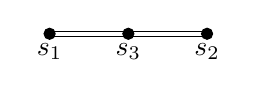
\begin{tikzpicture}
    \node at (-1,0) [below] {$s_{1}$};
    \node at (0,0) [below] {$s_{3}$};
    \node at (1,0) [below] {$s_{2}$};
    \draw (-1,0.03) -- (0,0.03) -- (1,0.03);
    \draw (-1,-0.03) -- (0,-0.03) -- (1,-0.03);
    \filldraw[black] (-1,0) circle (2pt);
    \filldraw[black] (0,0) circle (2pt);
    \filldraw[black] (1,0) circle (2pt);
  \end{tikzpicture}
\end{center}

Each of the nodes of this diagram corresponds to a variable of $Z(s_{1},s_{2},s_{3})$. The fact that there are two bonds between each node means that the group of functional equations of $Z(s_{1},s_{2},s_{3})$ is infinite. Precisely, it is the affine symmetric group $\wtilde{S_{3}}$. The root system associated to $Z_{\chi}(s_{1},\ldots,s_{5})$ is the affine dihedral group $\wtilde{D_{4}}$ whose Dynkin diagram is the following:
\begin{center}
  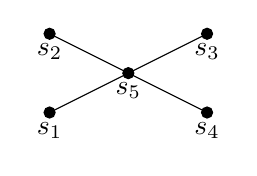
\begin{tikzpicture}
    \node at (-1,-0.5) [below] {$s_{1}$};
    \node at (-1,0.5) [below] {$s_{2}$};
    \node at (0,0) [below] {$s_{5}$};
    \node at (1,-0.5) [below] {$s_{4}$};
    \node at (1,0.5) [below] {$s_{3}$};
    \draw (-1,-0.5) -- (0,0);
    \draw (-1,0.5) -- (0,0);
    \draw (1,-0.5) -- (0,0);
    \draw (1,0.5) -- (0,0);
    \filldraw[black] (-1,-0.5) circle (2pt);
    \filldraw[black] (-1,0.5) circle (2pt);
    \filldraw[black] (1,-0.5) circle (2pt);
    \filldraw[black] (1,0.5) circle (2pt);
    \filldraw[black] (0,0) circle (2pt);
  \end{tikzpicture}
\end{center}
Notice that upon identifying the $s_{1}$ and $s_{2}$ nodes and the $s_{3}$ and $s_{4}$ nodes respectively, we recover the Dynkin diagram for $Z(s_{1},s_{2},s_{3})$. This is a geometric realization of the fact that
\[
  Z(s_{1},s_{2},s_{3}) \quad \text{and} \quad Z_{\chi}(s_{1},s_{1},s_{2},s_{2},s_{3}),
\]
have similar symmetry properties. In \cite{DIPP}, a generalized Chinta-Gunnells action was described that can be used to build a multiple Dirichlet series $Z_{\wtilde{C_{2}}}(s_{1},s_{2},s_{3})$ whose group of functional equations is isomorphic to $\wtilde{C_{2}}$. This series is analgous to that of the role of $Z_{\wtilde{D_{4}}}(s_{1},\ldots,s_{5})$. In a 2014 thesis of Whitehead (see \cite{W}), it was shown that for each affine Weyl group $W$ there exists a unqiue series $Z_{W}$ (up to a diagional term) satisfying certain growth properties and a group of functional equations isomorphic to $W$ when $W$ is \textit{simply laced}. The root system of type $\wtilde{C_{2}}$ is not simply laced, yet the generalized Chinta-Gunnells action is amenable to the ideas presented in Whitehead's thesis. Accordingly, $Z_{\wtilde{C_{2}}}(s_{1},s_{2},s_{3})$ is the \textit{unique} series (up to a diagional term) satisfying certain growth properties and a group of functional equations isomorphic to $\wtilde{C_{2}}$. This implies immediately that
\[
  Z_{\wtilde{C_{2}}}(s_{1},s_{2},s_{3}) = Z_{\wtilde{D_{4}}}(s_{1},s_{1},s_{2},s_{2},s_{3}),
\]
and therefore $Z_{\wtilde{C_{2}}}(s_{1},s_{2},s_{3})$ admits analytic continuation up to its natural barrier at $2s_{1}+2s_{2}+2s_{3} = -1$. The remaining question is how to express $Z(s_{1},s_{2},s_{3})$ in terms of $Z_{\wtilde{C_{2}}}(s_{1},s_{2},s_{3})$. Precisely, we are looking for an identity similar to \cref{equ:factorization}. To acomplish this, we expand $Z_{\wtilde{C_{2}}}(s_{1},s_{2},s_{3})$ into a Dirichlet series of shape
\[
  Z_{\wtilde{C_{2}}}(s_{1},s_{2},s_{3};q) = 1+\sum_{(k_{1},k_{2},k_{3}) \in \N^{3}-\{\mathbf{0}\}}a(k_{1},k_{2},k_{3};q)q^{-s_{1}k_{1}}q^{-s_{2}k_{2}}q^{-s_{3}k_{3}}.
\]
We at last define the multiple Dirichlet series
\[
  Z(s_{1},s_{2},s_{3}) = \sum_{m_{1},m_{2},d}\frac{a_{1}(m_{1})\chi_{d}(m_{1})a_{2}(m_{2})\chi_{d}(m_{2})A(m_{1},m_{2},d)}{|m_{1}|^{s_{1}}|m_{2}|^{s_{2}}|d|^{s_{3}}},
\]
where $a_{i}(m_{1})\chi_{d}(m_{i})$ are the coefficients of $L(s,E_{i} \x \chi_{d})$ and the coefficients $A(m_{1},m_{2},d)$ satisfy a twisted multiplicative property and are defined on primes by
\[
  A(p^{k_{1}},p^{k_{2}},p^{l}) = a\left(k_{1},k_{2},l;q^{-\frac{\deg(p)}{2}}\right). 
\]
We can apply the procedure in \cite{D} to sum up the series over $m_{1}$ and $m_{2}$ obtaining
\[
  Z(s_{1},s_{2},s_{3}) =  \sum_{d}\frac{L(s_{1},E_{1} \x \chi_{d})L(s_{2},E_{2} \x \chi_{d})P_{d}(s_{1},s_{2};E_{1},E_{2})}{|d|^{s_{3}}},
\]
where the correction polynomials $P_{d}(s_{1},s_{2};E_{1},E_{2})$ are now explicitly defined in terms of the $A(p^{k_{1}},p^{k_{2}},p^{l})$. This series satisfies a group of functional equations isomorphic to $\wtilde{C_{2}}$ where the functional equations are induced from those of $L(s_{i},E_{i} \x \chi_{d})$. By the uniqueness of $Z_{\wtilde{C_{2}}}$, it follows that there is a function $G$ in the variable $q^{-2s_{1}-2s_{2}-2s_{3}}$ such that
\[
  Z(s_{1},s_{2},s_{3}) = G(q^{-2s_{1}-2s_{2}-2s_{3}})Z_{\wtilde{C_{2}}}(s_{1},s_{2},s_{3}).
\]
The analytic continuation will be furnished if $G$ is is a holomorphic function. To see that it is, we take a residue at $s_{3} = 1$. This is possible since the series $Z_{\wtilde{C_{2}}}$ admits analytic continuation to the natural barrier. Upon taking this residue...

\textbf{Broader Impacts}:

\begin{thebibliography}{}
  \bibitem{BW}
  Friedberg, Solomon, ed. Multiple Dirichlet Series, Automorphic Forms, and Analytic Number Theory: Proceedings of the Bretton Woods Workshop on Multiple Dirichlet Series, Bretton Woods, New Hampshire, July 11-14, 2005. Vol. 75. American Mathematical Soc., 2006.

  \bibitem{Da}
  Davenport, Harold. Multiplicative number theory. Vol. 74. Springer Science \& Business Media, 2013.

  \bibitem{D}
  Diaconu, Adrian. "On the third moment of $L(\frac{1}{2},\chi_{d})$ I: The rational function field case." Journal of Number Theory 198 (2019): 1-42.

  \bibitem{DIPP}
  Diaconu, Adrian, et al. "Residues of quadratic Weyl group multiple Dirichlet series." arXiv preprint arXiv:2307.06223 (2023).

  \bibitem{DPP}
  Diaconu, Adrian, Vicentiu Pasol, and A. Popa. "Quadratic Weyl group multiple Dirichlet series of Type $D_{4}^{(1)}$." arXiv preprint arXiv:2111.11062.

  \bibitem{GH}
  Goldfeld, Dorian, and Jeffrey Hoffstein. "Eisenstein series of $\frac{1}{2}$-integral weight and the mean value of real Dirichlet $L$-series." Inventiones mathematicae 80.2 (1985): 185-208.

  \bibitem{M}
  Murty, M. Ram, and V. Kumar Murty. Non-vanishing of $L$-functions and applications. Springer Science \& Business Media, 2012.

  \bibitem{W}
  Whitehead, Ian. Multiple Dirichlet series for affine Weyl groups. Columbia University, 2014.

\end{thebibliography}
\end{document}